\section{Homotopies}  

\subsection{Homotopy} 

  Intuitively, a homotopy means that we can interpolate between $f_0$ and $f_1$ with a family of continuous maps $f_t$ varying continuously as a function of $t$. Sometimes, we slightly modify the definition a homotopy by restricting the family of continuous functions to agree on a certain subset $A$. We present both definitions below. 

  \begin{definition}[Homotopy]
    Let $X$ and $Y$ be topological spaces, with $f_0, f_1: X \to Y$ continuous. Then, a \textbf{homotopy} between $f_0$ and $f_1$ is a continuous map 
    \begin{equation}
      F: X \times [0, 1] \to Y
    \end{equation}
    such that $F(x, 0) = f_0 (x)$ and $f(x, 1) = f_1 (x)$ for all $x \in X$. In this case, we say $f_0$ and $f_1$ are \textbf{homotopic}, written $f_0 \simeq f_1$. 

    \begin{figure}[H]
      \centering 
      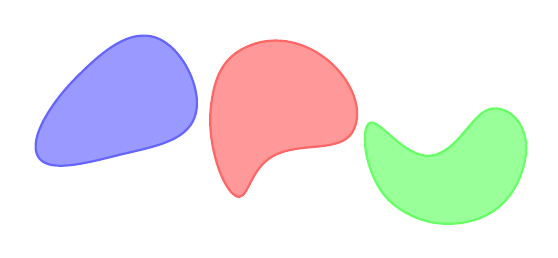
\begin{tikzpicture}
        % first blob (using random smooth cycle)
        \draw[fill=blue!40, draw=blue!60, thick] 
          plot[smooth cycle, tension=0.8] 
          coordinates {(0,0) (1,0.5) (0.5,1.5) (-0.5,1) (-1,0)};
        
        % second blob (using random smooth cycle)
        \draw[fill=red!40, draw=red!60, thick, xshift=2cm] 
          plot[smooth cycle, tension=0.8] 
          coordinates {(0,0) (1,0.3) (0.7,1.2) (-0.3,1.4) (-0.8,0.6) (-0.5,-0.5)};
        
        % third blob (using random smooth cycle)
        \draw[fill=green!40, draw=green!60, thick, xshift=4cm] 
          plot[smooth cycle, tension=0.8] 
          coordinates {(0,0) (0.8,0.6) (1.2,0) (0.6,-0.8) (-0.5,-0.6) (-0.8,0.4)};
      \end{tikzpicture}
      \caption{Think of the blobs as images of a certain function residing in $Y$. They are changing continuously. }
      \label{fig:single_homotopy_class}
    \end{figure}

    Given spaces $X, Y$ with $A \subset X, Y$ and $f_0, f_1 : X \to Y$ continuous maps such that $f_0 |_A = f_1 |_A$. A \textbf{homotopy relative to $A$} between $f_0$ and $f_1$ is a homtopy $F$ with the additional property that 
    \begin{equation}
      F(a, t) = f_0 (a, t) = f_1 (a, t) 
    \end{equation} 
    for all $a \in A, t \in I$. This is an equivalence relation. 
  \end{definition}
  \begin{proof}
    We prove that this is an equivalence relation. 
    \begin{enumerate}
      \item \textit{Reflexive}. Take $F(x, t) = f(x)$. 
      \item \textit{Symmetric}. If $f_0 \simeq f_1$ via homotopy $F$, then $G(x, t) = F(x, 1 - t)$ is a homotopy from $f_1$ to $f_0$. 
      \item \textit{Transitive}. If $f_0 \simeq f_1$ via $F$ and $f_1 \simeq f_2$ via $G$, then we define a new function 
        \begin{equation}
          H(x, t) \coloneqq \begin{cases} 
            F(x, 2t)  & \text{ if } 0 \leq t \leq \frac{1}{2} \\ 
            G(x, 2t - 1) & \text{ if } \frac{1}{2} \leq t \leq 1 
          \end{cases}
        \end{equation}
        which is continuous by the pasting lemma\footnote{The maps $t \mapsto F(x, 2t)$ and $t \mapsto G(x, 2t - 1)$ are continuous on the closed domains $X \times [0, \frac{1}{2}]$ and $X \times [\frac{1}{2}, 1]$ that coincide on $X \times \{\frac{1}{2}\}$.} and so is a homotopy. 
    \end{enumerate}
  \end{proof} 

  \begin{example}[Functions Mapping to Convex Spaces are Null-Homotopic]
    If $Y = \mathbb{R}^n$, then for any space $X$, any two continuous maps $f_0, f_1: X \to \mathbb{R}^n$ are homotopic by defining 
    \begin{equation}
      F(x, t) = (1 - t) f_0 (x) + t f_1 (x) 
    \end{equation}
    which is well-defined as $Y$ is convex. Furthermore, it is path connected, and so the value of the constant function does not matter. Any two constant functions are homotopic. 
  \end{example}

  \begin{example}[Two Non-Homotopic Functions]
    Consider $X = S^1, Y = \mathbb{R}^2 \setminus \{0\}$, with $f: S^1 \to Y$ the canonical inclusion, and $g$ any constant map. Then the straight line homotopy no longer works, since the circle gets ``stuck'' on the hole. That gives some sort of rigorous definition of what a hole can be. 
  \end{example}

  However, note that if two functions are null-homotopic, it \textit{does not} mean that they are homotopic to each other. 

  \begin{example}[Null-Homotopic Paths are Not Homotopic]
    Given $X = \mathbb{R}, Y = (0, 1) \cup (2, 3)$, say that we are given the functions $f, g: X \to Y$ defined $f(x) = 0.5, f(y) = 2.5$. Then by definition they are null-homotopic, but they are not homotopic to each other. 
  \end{example}

  This gives us a clue that if a space is path connected, then null-homotopic functions are homotopic to each other. We will elaborate on this later. The most fundamental way to construct new homotopies from old ones is by composing them with continuous functions. We can do this either before or after the homotopy. 

  \begin{lemma}[Continuous Compositions of Homotopic Maps are Homotopic]
    Let $f_0, f_1: X \to Y$ be continuous maps with $f_0 \simeq_A f_1$. 
    \begin{enumerate}
      \item If $g: Y \to Z$ is continuous, then $g \circ f_0 \simeq_A g \circ f_1$. 
      \item If $h: W \to X$ is continuous, then $f_0 \circ h \simeq_{h^{-1}(A)} f_1 \circ h$. 
    \end{enumerate}
  \end{lemma}
  \begin{proof}
    $f_0 \simeq f_1$ implies that  there is a homotopy 
    \begin{equation}
      F: X \times [0, 1] \to Y
    \end{equation}
    s.t. $F(x, 0) = f_0 (x), F(x, 1) = f_1 (x)$. 
    \begin{enumerate}
      \item Now we construct the map 
        \begin{equation}
          G = g \circ F : X \times [0, 1] \to Z
        \end{equation}
        Then, $g$ continuous implies $G$ is continuous, and we have 
        \begin{align}
          G(x, 0) & = (g \circ F)(x, 0) = g(f_0(x)) = (g \circ f_0) (x) \\ 
          G(x, 1) & = (g \circ F)(x, 1) = g(f_1(x)) = (g \circ f_1) (x) 
        \end{align}
        which is by definition a homotopy. 
        
      \item Given $h: W \to X$ continuous, then $h \times \mathrm{id} : W \times [0, 1] \to X \times [0, 1]$ is continuous under the product topology, and so we define the continuous map 
        \begin{equation}
          H = F \circ (h \times \mathrm{id}): W \times [0, 1] \to YH
        \end{equation}
        which satisfies 
        \begin{align}
          H(x, 0) & =  (F \circ (h \times \mathrm{id})) (x, 0) = F(h(x), 0) = f_0(h(x)) = (f_0 \circ h) (x) \\ 
          H(x, 1) & =  (F \circ (h \times \mathrm{id})) (x, 1) = F(h(x), 1) = f_1(h(x)) = (f_1 \circ h) (x) 
        \end{align}
    \end{enumerate}
  \end{proof}

  Now we have seen that homotopies form an equivalence class. Now it turns out that under function compositions, homotopies are preserved, making homotopies a congruence class. 

  \begin{theorem}[Homotopies is a Congruence Relation Under Composition]
    Given $f_0, f_1: X \to Y$ and $g_0, g_1: Y \to Z$, 
    \begin{equation}
      f_0 \simeq f_1, g_0 \simeq g_1 \implies g_0 \circ f_0 \simeq g_1 \circ f_1 
    \end{equation}
  \end{theorem}
  \begin{proof}
    We have $F: [0, 1] \times X \to Y$ and $G: [0, 1] \times Y \to Z$. Then, we can simply define the component-wise composition of maps
    \begin{equation}
      G \circ (F \times \mathrm{id}): [0, 1] \times X \to Z, \qquad (G \circ (F \times \mathrm{id})) (t, x) \coloneqq G \big(t, F(t, x) \big)
    \end{equation} 
    which is continuous. Also, it is the case that 
    \begin{align}
      (G \circ F) (0, x) & = G\big(0, F(0, x) \big) = G (0, f_0 (x)) = g_0 (f_0 (x)) = (g_0 \circ f_0) (x) \\ 
      (G \circ F) (1, x) & = G\big(1, F(1, x) \big) = G (1, f_1 (x)) = g_1 (f_1 (x)) = (g_1 \circ f_1) (x) 
    \end{align}
    So this is indeed a homotopy between $g_0 \circ f_0 \simeq g_1 \circ f_1$. 
  \end{proof}

\subsection{Path Homotopies and the Fundamental Group}

  Now we limit our scope to closed paths, which will unlock a nice algebraic structure that we can analyze. This is the beginning of \textit{algebraic topology}. Remember that a continuous map $f: [0, 1] \to X$ with $f(0) = x_0, f(1) = x_1$ is called a \textit{path}. A path from $x$ to itself is called a \textit{loop} at $x$. 
  
  \begin{definition}[Path Homotopy]
    Given two paths $f_0, f_1: [0, 1] \to X$, a \textbf{path homotopy} is a homotopy relative to $\{0, 1\}$, i.e. a continuous map $F: [0, 1] \times [0, 1] \to X$ s.t. 
    \begin{align}
      f(s, 0) & = f_0 (s) && f(s, 1) = f_1 (s) \\ 
      f(0, t) & = x && f(1, t) = x
    \end{align}
    for all $s, t$.\footnote{Note that the first line is the regular homotopy conditions, while the second line is the ``relative to''.}
  \end{definition}

  A corollary of the theorem on continuous compositions is that any path is path homotopic to any reparameterization of the same path. 

  \begin{corollary}[Reparameterizations are Still Path Homotopic]
    Suppose that $g: [0, 1] \to [0, 1]$ is a continuous map with $g(0) = 0, g(1) = 1$. Let $f: [0, 1] \to X$ be a path, and $f^\prime = f \circ g$. Then $f \simeq_p f^\prime$. 
  \end{corollary}
  \begin{proof}
    We can take the homotopy 
    \begin{equation}
      G: [0, 1] \times [0, 1] \to [0, 1], \qquad G(s, t) \coloneqq (1 - t) g(s) + t s 
    \end{equation}
    This is a homotopy between $g$ and the identity map $[0, 1]$ relative the endpoints since $G(s, 0) = g(s)$ and $G(s, 1) = s$. Now we compose this with $f$ to get the new continuous map  
    \begin{equation}
      F = f \circ G: [0, 1] \times [0, 1] \to X, 
    \end{equation}
    where 
    \begin{align}
      F(s, 0) & = f(G(s, 0)) = f(g(s)) = (f \circ g)(s) \\ 
      F(s, 1) & = f(G(s, 1)) = f(s) = f(s)
    \end{align} 
    and so $f \circ g \simeq_p f$. 
  \end{proof}

  The goal here is to try and develop some sort of algebraic structure on these paths. Therefore, let us define the following binary operation.  

  \begin{definition}[Concatenation of Paths]
    Given two paths $f$ from $x_0$ to $x_1$, and $g$ from $x_1$ to $x_2$, we can obtain a path from $x_0$ to $x_2$ by defining the \textbf{concatenation} of the paths as 
    \begin{equation}
      (f \ast g) (s) \coloneqq \begin{cases} 
        f(2s) & \text{ if } 0 \leq s \leq \frac{1}{2} \\ 
        g(2s - 1) & \text{ if } \frac{1}{2} \leq s \leq 1
      \end{cases}
    \end{equation}
    This is indeed a path since it is continuous by the pasting lemma. 
  \end{definition}

  It turns out that homotopies---which was originally an equivalence relation---is actually a \textit{congruence relation} with respect to concatenation. 

  \begin{lemma}[Path Homotopies is a Congruence Relation Under Concatenation]
    if $f_0, f_1$ are paths from $x_0$ to $x_1$, and $g_0, g_1$ are paths from $x_1$ to $x_2$, then 
    \begin{equation}
      f_0 \simeq_p f_1, g_0 \simeq_p g_1 \implies f_0 \ast g_0 \simeq_p f_1 \ast g_1
    \end{equation}
  \end{lemma}
  \begin{proof}
    Suppose $F$ and $G$ are path homotopies from $f_0$ to $f_1$ and $g_0$ to $g_1$. Then, we can define the ``concatenation'' of homotopies as the map
    \begin{equation}
      H(s, t) \coloneqq \begin{cases} 
        F(2s, t) & \text{ if } 0 \leq s \leq \frac{1}{2} \\ 
        G(2s - 1, t) & \text{ if } \frac{1}{2} \leq s \leq 1 
      \end{cases}
    \end{equation}
    Since they overlap on a closed set, then by the pasting lemma $H$ is continuous. Furthermore, we can see that 
    \begin{align}
      H(s, 0) & = F(0, t) = f_0 (s) = (f_0 \ast g_0) (s) \\ 
      H(s, 1) & = G(1, t) = g_1 (s) = (f_1 \ast g_1) (s) 
    \end{align}
  \end{proof}

  \begin{definition}[Fundamental Group]
    We denote by $\pi_1 (X, x_0)$ as the set of path homotopy classes of loops $[f]$ based at $x_0$. This, along with the binary operation. 
    \begin{equation}
      [f] \ast [g] \coloneqq [f \ast g] 
    \end{equation}
    and inverses is simply $[f]^{-1} \coloneqq [f^{-1}]$ where $f^{-1} (s) = f(1 - s)$. 
  \end{definition}
  \begin{proof}
    We prove the group axioms. 
    \begin{enumerate}
      \item \textit{Closure}. This is proved since path homotopies is a congruence relation under concatenation. 
      \item \textit{Associativity}. We prove something a bit more general. Let $f, g, h$ be paths from $x_0$ to $x_1$ to $x_2$ to $x_3$, respectively.  It is not the vase that $(f \ast g) \ast h = f \ast (g \ast h)$ since $\big( \frac{1}{4}, \frac{1}{4}, \frac{1}{2} \big) \neq \big( \frac{1}{2}, \frac{1}{4}, \frac{1}{4} \big)$. But they are reparamaterizations of each other, where $\varphi$ is some monotonically increasing continuous function from $[0, 1]$ to itself. Reparameterizations are path homotopic, and therefore 
        \begin{equation}
          ([f] \ast [g]) \ast [h] = [h] \ast ([g] \ast [h]) 
        \end{equation}

      \item \textit{Identity}. We claim that the constant path at $x_0$ (or more formally, the set of all null-homotopic paths at $x_0$) is the identity element. Since $e_{x_0}: [0, 1] \to X$ is defined $e_{x_0} (x) = x_{0}$, we have established that 
        \begin{equation}
          e_{x_0} \ast f \simeq_p f, \qquad f \ast e_{x_0} \simeq_p f
        \end{equation}

      \item \textit{Inverses}. If $f$ is a path from $x_0$ to $x_1$, then define $\bar{f} \coloneqq f(1 - x)$, which is a path from $x_1$  to $x_0$. Note that $f \ast \bar{f}$ is not the constant path $e_{x_0}$, but it is homotopic since 
        \begin{equation}
          (f \ast \bar{f}) (s) \coloneqq \begin{cases} 
            f(2s) = f(2s) & \text{ if } 0 \leq s \leq \frac{1}{2} \\ 
            \bar{f}(2s - 1) = f(2 - 2s) & \text{ if } \frac{1}{2} \leq s \leq 1
          \end{cases}
        \end{equation}
        But we use a sneaky trick and note that $p: [0, 1] \to [0, 1]$ defined as 
        \begin{equation}
          p(s) \coloneqq \begin{cases} 
            2s & \text{ if } 0 \leq s \leq \frac{1}{2} \\ 
            2 - 2s & \text{ if } \frac{1}{2} \leq s \leq 1
          \end{cases}
        \end{equation}
        satisfies $p(0) = p(1) = 0$, which implies that $p$ is homotopic to a constant path at $0$, which implies that $f \ast p$ is also null-homotopic. 
    \end{enumerate}
  \end{proof}

  Note that the identity element of $\pi_1 (X, x_0)$ is the \textit{constant} map $x \mapsto x_0$, not the identity map! This is different from a group of transformations. 

\subsection{Homomorphisms of Fundamental Groups}

  Now that we have constructed the fundamental group at a point $x_0$, the next things to consider are their behavior under group homomorphisms, and how different fundamental groups at different points (of the same topological space) look like. 

  \begin{definition}[Induced Group Homomorphism]
    Suppose $k: X \to Y$ is a continuous map with $x_0 \in X, y_0 = f(x_0) \in Y$. Define the map, called the \textbf{induced group homomorphism} of $k$ as 
    \begin{equation}
      k_\ast : \pi_1 (X, x_0) \to \pi_1 (Y, y_0), \qquad k_\ast ([f]) \coloneqq [k \circ f] 
    \end{equation}
    which is well defined since $f \simeq_p f^\prime$ in $X \implies k \circ f \simeq_p k \circ f^\prime$ in $Y$ as a composition with continuous functions. This is indeed a group homomorphism. 
  \end{definition}
  \begin{proof}
    Let's take a look at $f, g: [0, 1] \to X$. Then 
    \begin{equation}
      f \ast g : [0, 1] \to X, \qquad (f \ast g)(t) \coloneqq 
      \begin{cases} 
        f(2t)  & \text{ if } 0 \leq t \leq \frac{1}{2} \\ 
        g(2t - 1) & \text{ if } \frac{1}{2} \leq t \leq 1
      \end{cases}
    \end{equation}
    Therefore, mapping this through $k_\ast$ gives us 
    \begin{equation}
      k \circ (f \ast g) : [0, 1] \to Y, \qquad (k \circ (f \ast g)) (t) \coloneqq
      \begin{cases} 
        (k \circ f)(2t)  & \text{ if } 0 \leq t \leq \frac{1}{2} \\ 
        (k \circ g)(2t - 1) & \text{ if } \frac{1}{2} \leq t \leq 1
      \end{cases}
    \end{equation}
    Now take $k \circ f, k \circ g: [0, 1] \to Y$, and we can construct 
    \begin{equation}
      (k \circ f) \ast (k \circ g) : [0, 1] \to Y, \qquad \big( (k \circ f) \ast (k \circ g) \big) = \begin{cases} 
        (k \circ f) (2t) & \text{ if } 0 \leq t \leq \frac{1}{2} \\ 
        (k \circ g) (2t - 1) & \text{ if } \frac{1}{2} \leq t \leq 1
      \end{cases}
    \end{equation}
    which matches. Therefore we have $k \circ (f \ast g) = (k \circ f) \ast (k \circ g)$, and so under the congruence class 
    \begin{equation}
      k_\ast ([f] \ast [g]) = k_\ast([f \ast g]) = [k \circ f] \ast [k \circ g] = k_\ast ([f]) \ast k_\ast ([g]) 
    \end{equation}
  \end{proof}

  \begin{lemma}[Identity Map Induces Identity Group Homomorphism]
    If the continuous map between topological spaces is $k = \mathrm{id}_X$, then the induced homomorphism is simply the identity isomorphism. 
    \begin{equation}
      (\mathrm{id}_X)_\ast = (\mathrm{id}_{\pi_1 (X, x_0)}) 
    \end{equation}
  \end{lemma}
  \begin{proof}
    Just substituting with the formula above gives 
    \begin{equation}
      k_\ast ([f] \ast [g]) = [f] \ast [g] 
    \end{equation}
    and so $k_\ast$ must be the identity. 
  \end{proof}

  \begin{theorem}[Composition of Induced Group Homomorphisms]
    If $k: X \to Y$ and $l: Y \to Z$ are continuous, then 
    \begin{equation}
      (l \circ k)_\ast = l_\ast \circ k_\ast
    \end{equation}
  \end{theorem}
  \begin{proof}
    We have 
    \begin{align}
      (l \circ k)_\ast ([f]) & = [(l \circ k) \circ f ] \\ 
                             & = [l \circ  (k \circ f)] \\ 
                             & = l_\ast ([k \circ f]) \\ 
                             & = l_\ast (k_\ast ([f])) \\ 
                             & = (l_\ast \circ k_\ast) ([f]) 
    \end{align}
  \end{proof}

  \begin{corollary}[Homeomorphisms Induce Fundamental Group Isomorphisms]
    If $X \cong Y$ by a homeomorphism taking $x_0$ to $y_0$, then $\pi_1 (X, x_0) \cong \pi_1 (Y, y_0)$. 
  \end{corollary}
  \begin{proof}
    If $k: X \to Y$ is a homeomorphism, then $k: Y \to X$ is also a homeomorphism, both continuous. Then this induces the group homomorphisms $k_\ast: \pi_1 (X, x_0) \to \pi_1 (Y, y_0)$ and $k^{-1}_\ast: \pi_1 (Y, y_0) \to \pi_1 (X, x_0)$, and so from the lemma, 
    \begin{equation}
      k^{-1} \circ k = \mathrm{id}_X \implies (k^{-1} \circ k)_\ast = \mathrm{id}_{\pi_1 (X, x_0)}
    \end{equation}
    and so $(k^{-1})_\ast \circ k_\ast = \mathrm{id}_{\pi_1 (X, x_0)}$ and $k_\ast \circ (k^{-1})_\ast = \id_{\pi_1 (Y, y_0)}$. 
  \end{proof}

  Finally, let's talk about constructing new groups from old ones. 

  \begin{theorem}[Direct Products of Fundamental Groups]
    For any spaces $X, Y$, we have 
    \begin{equation}
      \pi_1 (X \times Y, x_0 \times y_0) \simeq \pi_1 (X, x_0) \times \pi_1 (Y, y_0)
    \end{equation}
    Moreover, the inclusion and projection maps on the topological spaces induce inclusion and projection maps on the groups. 
  \end{theorem}
  \begin{proof}
    A loop $f: I \to X \times Y$  with $f(0) = f(1) = (x_0, y_0)$ is the same as a pair of maps $f_X : I \to X$ and $f_Y : I \to Y$. A homotopy between loops is a continuous map $F: I \times I \to X \times Y$, which is the sames as a pair of homotopies $F_X$ and $F_Y$. 
  \end{proof}

  A fancy way to say this is that at every point, there is a group, and $\pi_1$ is a functor from the category of pointed topological spaces to the category of groups. 

\subsection{Simply Connected Spaces} 

  Now the final thing to mention for now is that there is a group at every single point in a topological space. They may be completely different groups, but the following theorem nicely categorizes them in terms of path components. 

  \begin{theorem}[Fundamental Groups of Points in a Path Component are Isomorphic]
    If $x_0$ and $x_1$ are on the same path component of $X$, then $\pi_1 (X, x_0) \simeq \pi_1 (X, x_1)$. The actual isomorphism depends on a choice of a path from $x_0$ to $x_1$. 
  \end{theorem}
  \begin{proof}
    Let $h$ be a path from $x_0$ to $x_1$, and let $f$ be a loop around $x_0$. We are given a loop in $x_0$ and want to essentially find a loop around $x_1$. We can define 
    \begin{equation}
      A_h : \pi_1 (X, x_0) \to \pi_1 (X_1, x_1), \qquad A_h([f]) \coloneqq [\bar{h} \ast f \ast h]
    \end{equation}
    Essentially, we want to start at $x_1$, go to $x_0$, loop around, and then go back to $x_1$, which is in total a loop around $x_1$. We claim that $A_h$ is an isomorphism by showing that it is a group homomorphism and that it has a well-defined inverse. 
    \begin{align}
      A_h ([f] \ast [g]) & = [\bar{h} \ast f \ast g \ast h] \\ 
                         & = [\bar{h} \ast f] \ast [g \ast h] \\ 
                         & = [\bar{h} \ast f] \ast [h \ast \bar{h}] \ast [g \ast h] \\ 
                         & = [\bar{h} \ast f \ast h] \ast [\bar{h} \ast g \ast h] \\ 
                         & = A_h ([f]) \ast A_h ([g]) 
    \end{align}
    As for inverses, TBD. 
  \end{proof}

  Of course, when $x_0$ and $x_1$ are in different path components, they may or may not have isomorphic fundamental groups. Therefore, when we know a space $X$ is path connected, we can just drop the point $x_0$ and just refer to the fundamental group as $\pi_1 (X)$. 

  Therefore, if the space is path connected, the fundamental group at all points are isomorphic. But even if all the groups are isomorphic, they may be nontrivial. This motivates the following definition. 
  
  \begin{definition}[Simply Connected Set]
    $X$ is called \textbf{simply connected} if it is path connected and $\pi_1 (X, x_0) = \{e\}$. 
  \end{definition}

  Note the following. 
  \begin{equation}
    \text{Simply Connected} \implies \text{Path Connected} \implies \text{Connected}
  \end{equation}

  \begin{example}[Simply Connected Spaces]
    The following are simply connected. 
    \begin{enumerate}
      \item $\mathbb{R}^n$ 
      \item Any convex subset of $\mathbb{R}^n$.
      \item Any star-shaped subset of $\mathbb{R}^n$, where a star-shaped set is defined as a set where there exists some point $x_0 \in A$ s.t. for all $y \in A$ the line segment from $x_0$ to $y$ is in $A$.  
    \end{enumerate}
  \end{example}

  \begin{lemma}
    If $X$ is simply connected, then any two paths $f, g$ connecting $x$ to $y$ are path-homotopic. 
  \end{lemma}
  \begin{proof}
    Given two paths $f, g$, then $f \ast \bar{g}$ is defined and is a loop of $X$ based at $x$. Since $X$ is simply connected, this is homotopic to the constant loop based at $x$. Then, 
    \begin{equation}
      [f] = [f \ast \bar{g}] \ast [g] = [e_x] \ast [g] = [g]
    \end{equation}
  \end{proof}

  \begin{theorem}[Union of Simply Connected Spaces]
    Suppose $X = U \cup V$, where $U, V$ are open and simply connected and $U \cap V$ is nonempty and path connected. Then $X$ is simply connected. 
  \end{theorem}
  \begin{proof}
    Let $x_0 \in U \cap V$. Given a loop $f$, we can factor $f$ as a composition $f = f_1 * \cdots * f_n$, where each $f_i$ is a path contained either in $U$ or in $V$, from some $x_{i-1} \in U \cap V$ to $x_i \in U \cap V$, and $x_n = x_0$. For $i = 1, \ldots, n-1$, choose a path $g_i$ from $x_0$ to $x_i$ in $U \cap V$.

    \begin{align}
      f &\simeq_p f_1 \overline{g}_1 g_1 f_2 \overline{g}_2 g_2 f_3 \ldots f_{n-1} \overline{g}_{n-1} g_{n-1} f_n\\
      &\simeq_p (f_1 \overline{g}_1)(g_1 f_2 \overline{g}_2)(g_2 f_3 \ldots f_{n-1} \overline{g}_{n-1})(g_{n-1} f_n)
    \end{align}

    Each of the factors is a loop in $U$ or $V$ based at $x_0$, so it can be contracted to $e_{x_0}$. Thus, $f \simeq e_{x_0}$, as required.
  \end{proof}

\subsection{Covering Maps}

  Now it turns out that a lot of sets are simply connected. So we will use this definition to categorize the fundamental groups of familiar spaces. However, the proofs of these requires the knowledge of covering spaces and lifts.  

  \begin{definition}[Covering Map]
    A function $p: Y \to X$ is a \textbf{covering map} if $p$ is 
    \begin{enumerate}
      \item surjective, 
      \item continuous, 
      \item and for every $x \in X$ there exists an open $U \ni x$ s.t. $p^{-1} (U) = \cup_\alpha V_\alpha$, where $V_\alpha$ are open and disjoint, and $p |_{V_\alpha}: V_\alpha \to U$ is a homeomorphism. 
    \end{enumerate}
    The sets $\{V_\alpha\}$ is a partition into \textbf{slices}, and $Y$ is said to be a \textbf{covering space} of $X$. 
  \end{definition}

  You can imagine a covering map as like a stack of pancakes $V_\alpha$ that get all squashed down to $U$. Now let's introduce a few properties of covering maps. 

  \begin{lemma}[Preimage of Singletons Have Discrete Topology]
    If $p: Y \to X$ is a covering map, then for each $x \in X$, the subspace $p^{-1} (x) \subset X$ has the discrete topology. 
  \end{lemma}
  \begin{proof}
    Take some $x \in X$ and look at its preimage $p^{-1}(x)$. Then, we can imagine it as some disjoint union of discrete points, which has the discrete topology. More formally, take some open $U \ni x$ and then its preimage will be the disjoint union of open sets $\sqcup_\alpha V_\alpha$. But each point $y \in p^{-1} (x)$ will be contained in exactly one of the $U_\alpha$'s, and so $y = y \cap U_\alpha$ is open in itself, meaning that all the $\{y_\alpha\}$ will have the discrete topology. 
  \end{proof} 

  \begin{theorem}[Covering Maps are Open Maps]
    If $p: Y \to X$ is a covering map, then it is open, i.e. maps open sets to open sets. 
  \end{theorem}
  \begin{proof}
    Suppose $A \subset Y$ is open. We wish to show that $p(A)$ is open. Choose an arbitrary $x \in p(A)$. By definition of covering maps, there must exist an open $U \ni x$ (but $U$ not necessarily in $p(A)$) s.t. $p^{-1} (U) = \sqcup_\alpha V_\alpha$ for $V_\alpha$ open. There is a point $y \in U$ s.t. $p(y) = x$. Let $U_\beta$ be the open slice containing $y$. Then, since $A$ is open by assumption, the set $V_\beta \cap A$ is open in $Y$ and hence open in $V_\beta$. Since $p$ maps $V_\beta$ homeomorphically onto $U$, it maps open sets to open sets and so $p(V_\beta \cap A)$ is open in $U$ and hence open in $X$. Furthermore, it is a neighborhood of $x$ contained in $p(A)$. Since for every $x \in p(A)$ has an open neighborhood contained in $p(A)$, $p(A)$ is thus open. 
  \end{proof}

  \begin{corollary}[Covering Maps are Quotient Maps]
    A covering map $p: Y \to X$ is a quotient map. 
  \end{corollary}
  \begin{proof}
    This is immediate because open maps are quotient maps.\footnote{However, open doesn't mean closed!} 
  \end{proof}

  \begin{example}[Reals to the Circle]
    The following is a covering map. 
    \begin{equation}
      p: \mathbb{R} \to S^1, \qquad p(t) = (\sin{2 \pi t}, \cos{2 \pi t})
    \end{equation}
    It is clearly surjective and continuous. Now given any $x \in S^1$, let's take the open neighborhood $U \ni x$. Then, its preimage is the union of disjoint intervals $V_n$ for $n \in \mathbb{N}$, and if we restrict it to each $V_n$, then it is a homeomorphism. 
  \end{example}

  \begin{example}[Positive Reals to the Circle]
    The map 
    \begin{equation}
      p: \mathbb{R}^+ \to S^1, \qquad p(x) \coloneqq ( \cos{2 \pi x}, \sin{2\pi x}) 
    \end{equation}
    is not a covering map. It is surjective and continuous but the point $x_0 = (1, 0) \in S^1$ has no neighborhood $U$ that is evenly covered by $p$. We can see that the inverse image of $(0, \epsilon)$ is not homeomorphic to an open $U$. 
  \end{example}

  These examples might lead you to think that $\mathbb{R}$ is the only connected covering space of $S^1$. It turns out that a space can be a covering space of itself. 

  \begin{example}[Covering Map of $S^1$ to Itself]
    We can consider $S^1 \subset \mathbb{C}$ and claim that the following is a covering map. 
    \begin{equation}
      p: S^1 \to S^1, \qquad p(z) = z^2
    \end{equation}
  \end{example}

  \begin{theorem}[Restriction of Covering Maps]
    Let $p: Y \to X$ be a covering map. If $Y_0 \subset Y$ and $X_0 = p^{-1}  (Y_0)$, then the restriction $p_0: Y_0 \to X_0$ is a covering map. 
  \end{theorem}
  \begin{proof}
    Given $x_0 \in X_0$, let $U \ni x_0$ be an open set. Then let $\{V_\alpha\}$ be a partition of $p^{-1} (U)$ into slices. We know that $U \cap X_0$ is an open neighborhood of $x_0$ in $X_0$, and taking the preimage we have 
    \begin{equation}
      p^{-1} (U \cap X_0) = \sqcup_\alpha V_\alpha \cap p^{-1} (X_0) = \sqcup_\alpha V_\alpha \cap Y_0
    \end{equation}
    The $V_\alpha \cap Y_0$ are disjoint, and $V_\alpha$ open in $Y$ implies that $V_\alpha \cap Y_0$ is open in $Y_0$. Finally, we can see that $p$ maps $V_\alpha$ homeomorphically onto $U$, and so $p$ maps $V_\alpha \cap Y_0$ homeomorphically onto $p(V_\alpha) \cap p(Y_0) = U \cap X_0$. 
  \end{proof}

  \begin{theorem}[Product of Covering Maps]
    If $p: Y \to X$ and $p^\prime : Y^\prime \to X^\prime$ are covering maps, then 
    \begin{equation}
      p \times p^\prime : X \times X^\prime \to Y \times Y^\prime
    \end{equation}
    is a covering map. 
  \end{theorem}
  \begin{proof}
    Given $x \in X, x^\prime \in X^\prime$, let $U \ni x, U \ni x^\prime$ be open neighborhoods of $x$ and $x^\prime$ with $\{V_\alpha\}, \{V_\alpha^\prime\}$ the even slices of $p^{-1}, (p^\prime)^{-1}$. Then the preimage 
    \begin{equation}
      (p \times p^\prime)^{-1} (U \times U^\prime) = \bigcup_{\alpha, \beta} V_\alpha \times V_\beta^\prime 
    \end{equation}
    These are disjoint open sets of $X \times X^\prime$, each of which is mapped homeomorphically onto $U \times U^\prime$ by $p \times p^\prime$. 
  \end{proof}

  \begin{theorem}[Composition of Covering Maps]
    Let $q: X \to Y$ and $r: Y \to Z$ be covering maps. If $r^{-1}(z)$ is finite for all $z \in Z$, then $p = r \circ q: X \to Z$ is a covering map. 
  \end{theorem}
  \begin{proof}
    
  \end{proof}

  What we should keep in mind is that locally, covering maps look like homeomorphisms. 

  \begin{example}[Projection of Products with Discrete Topology]
    Let $Y$ have the discrete topology, and $p: X \times Y \to X$ is a projection on the first coordinate. Then we claim that $p$ is a covering map. Note that the open sets are of the form 
    \begin{equation}
      X \times \{y\} \text{ for } y \in Y
    \end{equation}
  \end{example}

  \begin{example}
    Say $k \in \mathbb{Z} \setminus \{0\}$ and $f_k : S^1 \to S^1$ defined 
    \begin{equation}
      f_k (\cos{\theta}, \sin{\theta}) \coloneqq (\cos{k \theta}, \sin{k\theta})
    \end{equation}
    This circularly stretches out the circle by a factor of $k$. We claim that this is a covering map. 
  \end{example}

  \begin{theorem}[Covering Maps as Homeomorphisms]
    Let $p: Y \to X$ be a covering map with $X$ simply connected and $Y$ path connected. Then $p$ is a homeomorphism. 
  \end{theorem}

\subsection{Lifts}
  
  There is a nice relationship between the fundamental group and the covering space. 

  \begin{definition}[Lift]
    If $p: Y \to X$ is a covering map and $f: Z \to X$ is continuous, then a \textbf{lift} of $f$ is a continuous map $\Tilde{f}: Z \to Y$ satisfying $p \circ \Tilde{f} = f$.\footnote{It is called a lift since it ``lifts'' the function with codomain $Z$ to the larger covering space $Y$.}

    \begin{figure}[H]
      \centering 
      \begin{tikzcd}
        & Y \arrow[d, "p"] \\
        Z \arrow[r, "f"] \arrow[ru, "\Tilde{f}"] & X
      \end{tikzcd}
      \caption{Commutative diagram of a lift.} 
      \label{fig:lift}
    \end{figure}
  \end{definition}

  Note that not every $f$ has a lift. However, it turns out that the existence of liftings when $p$ is a covering map is an important tool for studying covering spaces and the fundamental group. The path lifting property guarantees that paths can be lifted into a covering space. 

  \begin{lemma}[Path Lifting Property]
    Suppose $p: Y \to X$ is a covering map with $p(y_0) = x_0$. Given any path $f: [0, 1] \to X$ with $f(0) = x_0$, there exists a unique lift $\Tilde{f}: [0, 1] \to Y$ with $\Tilde{f}(0) = y_0$. 
  \end{lemma}

  Therefore, this essentially means that by taking the covering map $p$ that sends $y_0$ to $x_0$ and a path $f$ starting at $x_0$, we can construct a corresponding path $\Tilde{f}$ starting at $y_0$ such that $f = p \circ \Tilde{f}$. Let's do an example. 

  \begin{example}[Lift of Real Interval to $S^1$]
    Consider the covering map and path defined as below. 
    \begin{equation}
      p: \mathbb{R} \to S^1, \qquad p(t) = (\cos{2 \pi t}, \sin{2 \pi t}) 
    \end{equation}
    We can see that $p(y_0) = p(0) = (1, 0) = x_0$. Now let's consider a few paths $f: [0, 1] \to S^1$. We would like to ``lift'' this path $I \to S^1$ to a path $I \to \mathbb{R}$. The lemma states that there is indeed a unique path. 
    \begin{enumerate}
      \item When $f(s) = (\cos{\pi s}, \sin{\pi s})$ which satisfies $f(0) = x_0 = (1, 0)$, the lift is $\Tilde{f}(t) = t/2$ which satisfies $\Tilde{f}(0) = y_0 = 0$. 
      \begin{equation}
        t \xrightarrow{\Tilde{f}} \frac{t}{2} \xrightarrow{p} \big( \cos{2 \pi \frac{t}{2}}, \sin{2 \pi \frac{t}{2}} \big) = ( \cos{\pi t}, \sin{\pi t}) = f(t)
      \end{equation}

      \item When $f(s) = (\cos{\pi s}, -\sin{\pi s})$ which satisfies $f(0) = x_0 = (1, 0)$, the lift is $\Tilde{f}(t) = -t/2$ which satisfies $\Tilde{f}(0) = y_0 = 0$. 
      \begin{equation}
        t \xrightarrow{\Tilde{f}} -\frac{t}{2} \xrightarrow{p} \big( \cos{-2 \pi \frac{t}{2}}, \sin{-2 \pi \frac{t}{2}} \big) = ( \cos{\pi t}, \sin{-\pi t}) = f(t)
      \end{equation}
      since $\cos(t) = \cos(-t)$. 
    \end{enumerate}

    \begin{figure}[H]
      \centering 
      \begin{tikzcd}
        & \mathbb{R} \arrow[d, "p"] \\
        {[a, b]} \arrow[r, "f"] \arrow[ru, "\Tilde{f}"] & S^1
      \end{tikzcd}
      \caption{} 
      \label{fig:lift_ex}
    \end{figure}
  \end{example}

  Then, we show that path homotopies can be lifted as well. 

  \begin{lemma}[Homotopy Lifting Property]
    Suppose $p: Y \to X$ is a covering map. If $f, g: I \to X$ are paths with $f(0) = g(0), f(1) = g(1)$, and $f \simeq_p g$ (path homotopic), and $\Tilde{f}, \Tilde{g}: I \to Y$ are lifts starting at the same $y_0$, then $\Tilde{f} \simeq_p \Tilde{g}$. 
  \end{lemma}

  Great, so we have defined covering maps and have shown that paths admit lifts that are consistent with the path homotopy relation. Now, to connect this back to fundamental groups, we introduce the following theorem which allows us to determine the cardinality of fundamental groups through covering maps over simply connected spaces. This will be very useful to us later on.  

  \begin{theorem}[Bijection from Fundamental Group to Preimage of Covering Map on Simply Connected Space]
    If $p: Y \to X$ is a covering map and $Y$ is simply connected, then $\pi_1 (X, x_0)$ is in bijection with $p^{-1}(x_0)$. 
  \end{theorem} 
  \begin{proof}
    Given a loop $f: [0, 1] \to X$ with $f(0) = f(1) = x_0$, fix $y_0 \in p^{-1} (x_0)$. By the path lifting property, we can take the lifted path $\Tilde{f}: [0, 1] \to Y$ with $\Tilde{f}(0) = y_0$. 
    \begin{equation}
      p(\Tilde{f}(1)) = f(1) = y_0, \qquad \Tilde{f}(1) \in p^{-1} (x_0)
    \end{equation}
    By the homotopy lifting property, this only depends on $[f] \in \pi_1 (X, x_0)$. 
    \begin{enumerate}
      \item To prove surjectivity, since $Y$ is simply connected, this implies $Y$ is path connected. Choose a path $g$ from $y_0$ to $y$. Let $f = p \circ g$. Then $L([f]) = g(1) = y$. 

      \item To prove injectivity, if $L ([f]) = L([g])$, then $\Tilde{f}$ and $\Tilde{g}$ are both paths in $Y$ from $y_0$ to $y_1$. Because $Y$ is simply connected, $\Tilde{f} \simeq_p \Tilde{g} \implies f \simeq_p g \implies [f] = [g]$. 
    \end{enumerate}
  \end{proof}

  \begin{example}
    Take $p: \mathbb{R}^2 \to S^1 \times S^1$ defined 
    \begin{equation}
      (s, t) \mapsto \big( (\cos{2 \pi s}, \sin{2 \pi s}), (\cos{2 \pi t}, \sin{2 \pi t}) \big)
    \end{equation}
    Think back to the quotient space representation. 
    \begin{equation}
      T^2 = [0, 1]^2 /{\sim}, \qquad (x, 0) \sim (x, 1) \forall x, (0, y) \sim (1, y) \forall y
    \end{equation}
    Then we can think of $p(x, y) = (x \pmod{1}, y \pmod{1})$. We claim that this is a covering map. 
  \end{example}

\subsection{Fundamental Groups of Euclidean Space and the Sphere}

  Now that we have established that $\mathbb{R}^n$ is simply connected, along with some tools on sufficient conditions for simply connectedness and lifts, we can start to categorize fundamental groups of $\mathbb{R}^n$ and $S^n$, with the corresponding sets minus a point. 

  \begin{theorem}[Fundamental Groups of $S^n$]
    We have 
    \begin{enumerate}
      \item For $n = 1$, $S^1$ is path connected but not simply connected. 
        \begin{equation}
          \pi_1 (S^1) \simeq \mathbb{Z}
        \end{equation}

      \item For $n \geq 2$, $S^n$ is simply connected, and so 
        \begin{equation}
          \pi_1 (S^n) \simeq \{e\}
        \end{equation}
    \end{enumerate}
  \end{theorem}
  \begin{proof}
    Consider the map $p: \mathbb{R} \to S^1$ given by $t \mapsto (\cos{2 \pi t}, \sin{2 \pi t})$.\footnote{This is a classic example of what's called a covering map, which we will define later.} For each $x \in S^1$, there is an open set $U$ such that $p^{-1} (U)$ is a disjoint union of open sets $V_{i}$, where $p|_{V_i}$ is a homeomorphism. Let $x_0 = (1, 0)$. Then $p^{-1} (x_0) = \mathbb{Z}$. Then here are the key technical steps. 
    \begin{enumerate}
      \item For any continuous path $f: [0, 1] \to S^1$ with $f(0) = x_0$, and any choice of $\Tilde{x}_0 \in \mathbb{R}$ with $p(\Tilde{x_0}) = x_0$ (i.e. some integer), there is a unique continuous function $\Tilde{f}: [0, 1] \to \mathbb{R}$ with $f(0) = \Tilde{x_0}$. 
      \item $\Tilde{f}(1) - \Tilde{f}(0)$ measures the ``net winding'' of $f$. $1/2\pi$ times the net increase in the angle coordinate. In particular, if $f$ is a loop, then $\Tilde{f} (1) - \Tilde{f}(0)$ is an integer, which we'll call the \textit{winding number} of $f$, denoted $\omega (f)$. This doesn't depend on which choice of $\Tilde{f}$ we made. 
      \item Given two loops $f, g$ based at $x_0$, let $\Tilde{f}, \Tilde{g}$ by their lifts, with say $\Tilde{f}(0) = \Tilde{g}(0) = 0$. Then $f \simeq_p g$ iff $\Tilde{f} \simeq p \Tilde{g}$. One direction is easy. If $F$ is a path homotopy between $\Tilde{f}$ and $\Tilde{g}$, then $p \circ F$ is a path homotopy between $f$ and $g$. The other direction requires a somewhat elaborate argument using compactness. 
      \item As a consequence, we see that if $f \simeq_p g$, then $\Tilde{f} (1) = \Tilde{g} (1)$, and hence $\omega (f) = \omega(g)$. 
      \item Conversely, if $\omega(f) = \omega(g) = n$, then $\Tilde{f}$ and $\Tilde{g}$ are both paths in $\mathbb{R}$ from $0$ to $n$. There is a straight line homotopy between them. $F(s, t) = (1 - t) \Tilde{f} (s) + t \Tilde{g}(s)$. So $f \simeq_p g$. 
      \item We then have $\omega(f \ast g) = \omega(f) + \omega(g)$. 
      \item Thus, the winding number gives us an isomorphism from $\pi_1 (S^1) \to \mathbb{Z}$. 
    \end{enumerate}
    By using the function $p: \mathbb{R}_+ \times \mathbb{R} \to \mathbb{R}^2 \setminus \{0\}$, given by $p(r, t) = (r \cos{2 \pi t}, r \sin{2 \pi t})$, we can use the same logic. Another way to see it is that $\mathbb{R}^2 \setminus \{0\} \cong S^1 \times (0, \infty) \cong S^1 \times \mathbb{R}$. 
  \end{proof}

  Now we explore the fundamental groups of $S^n$ minus a point. This becomes very simple once we know the stereographic projection. 

  \begin{theorem}[Stereographic Projection]
    We claim 
    \begin{equation}
      S^n \setminus \{n\} \cong \mathbb{R}^{n}
    \end{equation}
  \end{theorem}
  \begin{proof}
    We can construct a formula, but visually, we can take any $x \in S^n \setminus \{n\}$, and there is a unique line $L$ through $x$ and $n$. Now let $f(x) \coloneqq L _x \cap (\mathbb{R}^{n-1} \times \{0\})$, which is bijective. It also turns out to be a homeomorphism. 
  \end{proof}

  \begin{corollary}[Fundamental Groups of $S^n$ Minus a Point]
    We claim that $S^n \setminus \{p\}$ is simply connected, for all $n \in \mathbb{N}$. 
    \begin{equation}
      \pi_1 (S^n) \simeq \{e\}
    \end{equation}
  \end{corollary}

  So informally, $S^n$ minus a point gives us $\mathbb{R}^n$, so what if we remove a point from $\mathbb{R}^n$? It turns out that by taking $n$ points away from $S^n$, it is equal to taking $n-1$ points away from $\mathbb{R}^n$. 

  \begin{theorem}[Fundamental Groups of $\mathbb{R}^n$ Minus a Point]
    We claim that 
    \begin{enumerate}
      \item For $n = 1$, $\mathbb{R} \setminus \{0\}$ is not even path connected. For any $x_0$, we have 
        \begin{equation}
          \pi_1 (\mathbb{R} \setminus \{0\}) \simeq \{e\}
        \end{equation}

      \item For $n = 2$, $\mathbb{R}^2 \setminus \{0\}$ is path connected, but it is not simply connected.\footnote{We can think of this as a hole in the middle of the plane that paths cannot unwind through.}
        \begin{equation}
          \pi_1(\mathbb{R}^2 \setminus \{x\}) \simeq \mathbb{Z}
        \end{equation}

      \item For $n \geq 3$, $\mathbb{R}^n \setminus \{x\}$ is simply connected.\footnote{We can interpret as if the extra dimensions being added gives more space for a path to unwind.}
    \end{enumerate}
  \end{theorem}
  \begin{proof}
    For $n = 1$, we can see that $(-\infty, 0)$ and $(0, +\infty)$ are convex subsets, so they are simply connected. For $n = 2$, we can see in polar coordinates, 
    \begin{equation}
      \mathbb{R}^2 \setminus \{0\} \simeq S^1 \times (0, +\infty) \implies \pi_1 (\mathbb{R}^2 \setminus \{0\}) \simeq \pi_1 (S^1) \times \pi_1 ((0, +\infty)) \simeq \mathbb{Z} \times \{e\} \simeq \mathbb{Z}
    \end{equation}
    For $n = 3$, we can construct it from smaller simply connected spaces. Take 
    \begin{align}
      U & = \mathbb{R}^n \setminus \{(0, \ldots, 0, z) \mid z \geq 0\} \\
      V & = \mathbb{R}^n \setminus \{(0, \ldots, 0, z) \mid z \leq 0\}
    \end{align}
    These are each open (since the axes that we minus out is closed) and simply connected (since they are star convex). Also, $U \cap V = (\mathbb{R}^{n-1} \setminus \{0\}) \times \mathbb{R}$, which is path connected since we assumed that $n \geq 3$. Therefore, by the theorem above, $\mathbb{R}^n \setminus \{0\}$ is simply connected. 
  \end{proof}

  \begin{theorem}[Fundamental Groups of $\mathbb{RP}^n$]
    We claim that. 
    \begin{enumerate}
      \item For $n = 1$, $\mathbb{RP}^1 \cong S^1$ and so $\pi_1(\mathbb{RP}) \simeq \mathbb{Z}$. 
      \item For $n \geq 2$, $\pi_1 (\mathbb{RP}^n) \simeq \mathbb{Z}_2$
    \end{enumerate}
  \end{theorem}
  \begin{proof}
    For $n = 1$, recall that $S^1$ is homeomorphic to $S^1/{\sim}$ where $x \sim -x$ through the homeomorhism $z \mapsto z^2$. 

    For $n \geq 2$, we claim that the projection map $p: S^n \to \mathbb{RP}^n$ defined $-\pm x \to x$ is a covering map. Furthermore, we know that $S^n$ is simply connected (since it's homeomorphic to $\mathbb{R}^n \setminus \{0\}$), and therefore there exists a bijection from $\pi(\mathbb{RP}^n, x_0)$ with $p^{-1} (x_0) = \{\pm x_0\}$. Therefore the order of the fundamental group must be $2$, and it can only be $\mathbb{Z}_2$ for all $x_0$. 
  \end{proof}

  At this point it's pretty easy to show the fundamental groups of familiar quotient spaces. 

  \begin{example}[Torus]
    The torus $T \cong S^1 \times S^1$ is path connected has the fundamental group 
    \begin{equation}
      \pi_1 (T) \simeq \pi_1 (S^1) \times \pi_1 (S^1) \simeq \mathbb{Z} \times \mathbb{Z}
    \end{equation}
    So it is not simply connected. 
  \end{example}

  \begin{example}[Cylinder]
    The cylinder is path connected and the fundamental group is 
    \begin{equation}
      \pi_1 (S^1 \times [0, 1]) \simeq \pi_1 (S^1) \times \pi_1 ([0, 1]) \simeq \mathbb{Z} \times \{e\} \simeq \mathbb{Z} 
    \end{equation}
  \end{example}

  \begin{example}[Mobius Strip]
    The Mobius strip is not simply connected. 
  \end{example}

  \begin{example}[Klein Bottle]
    The Klein bottle is not simply connected and it is not abelian. 
  \end{example}

\subsection{Retractions}

  \begin{definition}[Retraction]
    If $A \subset X$, a retraction $r: X \to A$ is a continuous function such that $r(a) = a$ for all $a \in A$.  
  \end{definition}

  \begin{example}
    The following are retractions. 
    \begin{equation}
      r: \mathbb{R} \to \{x\} \subset \mathbb{R}, \qquad r(x) = x
    \end{equation}
    This is also a retraction. 
    \begin{equation}
      r: \mathbb{R} \setminus \{0\} \to S^{n-1}, \qquad x \mapsto \frac{x}{\|x\|} 
    \end{equation}
  \end{example}

  \begin{lemma}[Group Homomorphism Induced By Retraction]
    Given $A \subset X$, a retraction $r: X \to A$, and the canonical injection $\iota: A \to X$, 
    \begin{enumerate}
      \item The induced homomorphism $r_\ast: \pi_1 (X, a_0) \to \pi_1 (A, a_0)$ is surjective. 
      \item The induced homomorphism $\iota_\ast: \pi_1 (A, a_0) \to \pi_1 (X, a_0)$ is injective. 
    \end{enumerate}
  \end{lemma}
  \begin{proof}
    
  \end{proof}

  It's pretty easy to show whether a particular example is a retraction or not. However, we will mainly be interested in the existence of retractions. 

  \begin{theorem}[Unit Interval to Endpoints]
    There is no retraction from $D^1 = [-1, 1]$ to $S^0 = \{-1, 1\}$. 
  \end{theorem}
  \begin{proof}
    Let $X = [a, b]$. There is no retraction $f: X \to \{a, b\}$ since $\im(f)$ must be connected. But $f(a) = a, f(b) = b$. Alternatively, we can use IVT. 
  \end{proof}

  \begin{theorem}[Unit Disk to Circular Boundary]
    There is no retraction from $D^2 \to S^1$. Intuitively, we can see that the mapping has to ``tear'' the disk somewhere!
  \end{theorem}
  \begin{proof}
    
  \end{proof}

  \begin{theorem}
    Let $A \subset X$, and $x_0 \in A$, and $r: X \to A$ be a retraction. Then the induced map $r_\ast: \pi_1 (X, x_0) \to \pi_1 (A, x_0)$ is surjective. 
  \end{theorem}
  \begin{proof}
    Given retraction $r: X \to A$ and the canonical injection $\iota: A \to X$, we have $r \circ \iota = \mathrm{id}_A$ by definition. Now see how it affects the fundamental spaces. 
    \begin{equation}
      \pi_1 (A, x_0) \xrightarrow{\iota_\ast} \pi_1 (X, x_0) \xrightarrow{r_\ast} \pi_1 (A, x_0)
    \end{equation}
    Therefore $r_\ast \circ \iota_\ast = \mathrm{id}_A$. So for any loop $[f] \in \pi_1 (A)$, $[f] = r_\ast (i_\ast ([f]))$, so $[f] \in \im(r_\ast)$. Also $\iota_\ast$ is injective. 
  \end{proof}

  \begin{corollary}
    If $X$ is simply connected and $A$ is not, then there is no retraction. 
  \end{corollary}

  Extending this a bit, remember that any continuous function $f: [a, b] \to [a, b]$ must have a fixed point by IVT. Thinking $D^1 = [-1, 1]$, we claim the following. Note that a rotation of the disk $D^2$ has a fixed point in the center. 

  \begin{theorem}[Brower's Fixed Point Theorem]
    Any continuous function $f: D^2 \to D^2$ has a fixed point, i.e. there exists $x \in D^2$ s.t. $f(x) = x$.\footnote{This was first proven in the 1930s based on a non-intersection theorem . But it is non-constructive, i.e. doesn't show you how to find the point. }
  \end{theorem}
  \begin{proof}
    Suppose $f: D^2 \to D^2$ has no fixed point. Define a function $g: D^2 \to D^2$ as follows. For $x$, take $f(x) \neq x$ and draw a ray from $f(x)$ to $x$ (directions matter!). Where it hits the boundary is the output $g(x)$. It is much more tedious to write out in formulas, but if you do, you can see that it's just the composition of continuous functions and is so continuous. If $x \in S^1$, then $g(x) = x$, so I've just constructed a retraction from $D^2$ to $S^1$, which is a contradiction! 
  \end{proof}

  So what about higher dimensions? If we believe that there is no retraction $D^n \to S^{n-1}$, by the same method we can prove for $D^n \to D^n$. The problem is that for $n \geq 2$ $S^{n-1}$ is simply connected and so $\pi_1(S^{n-1}) = \{e\}$, and same holds for $D^n$. So we can't prove the non-retraction using fundamental groups $\pi_1$. This is where we need higher order homotopy groups. 

